\section{Closing}



%%%%%%%%%%%%%%%%%%%%%%%%%%%%%%%%%%%%%%%%%%%%%%
% \begin{frame}[label=ladila]{Philosophy}

% KT sits naturally in the context of \textbf{panpsychism} (`mind is everywhere', see Strawson, \cite{Goff:2019aa}), a somewhat controversial version of the philosophy of consciousness.  \vfill

% \textbf{Idealism} is perhaps a more rigorous philosophical background (consciousness as the fundamental entity, `mind is everything'). \vfill

%  Although not necessary for the exploration of the scientific implications of the theory, the adoption of idealism can itself be motivated by simplicity and consistency criteria \citep{Symes2022-ri}.
 
% \end{frame}



%%%%%%%%%%%%%%%%%%%%%%%%%%%%%%%%%%%%%%%%%%%%%%
\begin{frame}[label=ladila]{Ethics}

KT does not grant any special status to humans:  all \textbf{agents} enjoy structured experience with  \textbf{pleasure/pain (valence)}. \vfill


The framework has other implications. E.g.,  \textit{morality}:  natural notions of {\em good} or {\em evil} in computational terms. \vfill

E.g., we may say that Agent's $A$ is \textbf{good} to Agent $B$ if the objective function   $O_A$ increases when O$_B$ increasing, that is $O_A(O_B)$ is increasing or  $O_A'(O_B) >0$ (and viceversa for \textbf{evil}).
 \vfill
 
% Conversely, we say that Agent $A$ is {\em good or morally right} to Agent $B$ if $O_A'(O_B) >0$. \vfill 

%Synergistic behavior emerges when agents are \textit{kind} to each other, while mutually-destructive behavior takes place in the complementary case.  
 
\end{frame}

%%%%%%%%%%%%%%%%%%%%%%%%%%%%%%%%%
\begin{frame}[label=ladila]{Future}
% Firmly reconcile KT with AIF/FEP, IIT, GWT, DIT. 
 % \vfill
 

Demonstrate how to computationally \textit{evolve agents}. KT conjecture: \textit{\textit{Under some conditions, persistent patterns} are unavoidable  in a computational soup if we wait long enough.} Are there patterns other than agents  (life/intelligence)? \vfill

How can we detect an agent through its behavior or structure? \vfill


How can we associate the structure of dynamical hierarchical reduced manifolds\cite{ruffini_algorithmic_2024} with first and third-person data?\vfill

Use AI to design better neurophenomenological methods to study \SEP.   \vfill

Map the neurobiology of agenthood\cite{ruffini_algorithmic_2024}?\vfill

Design model-building agents mimicking life or intelligence. 
 
\end{frame}


\begin{frame}{Call for papers: Special Entropy issue}

\begin{figure}
        \centering
        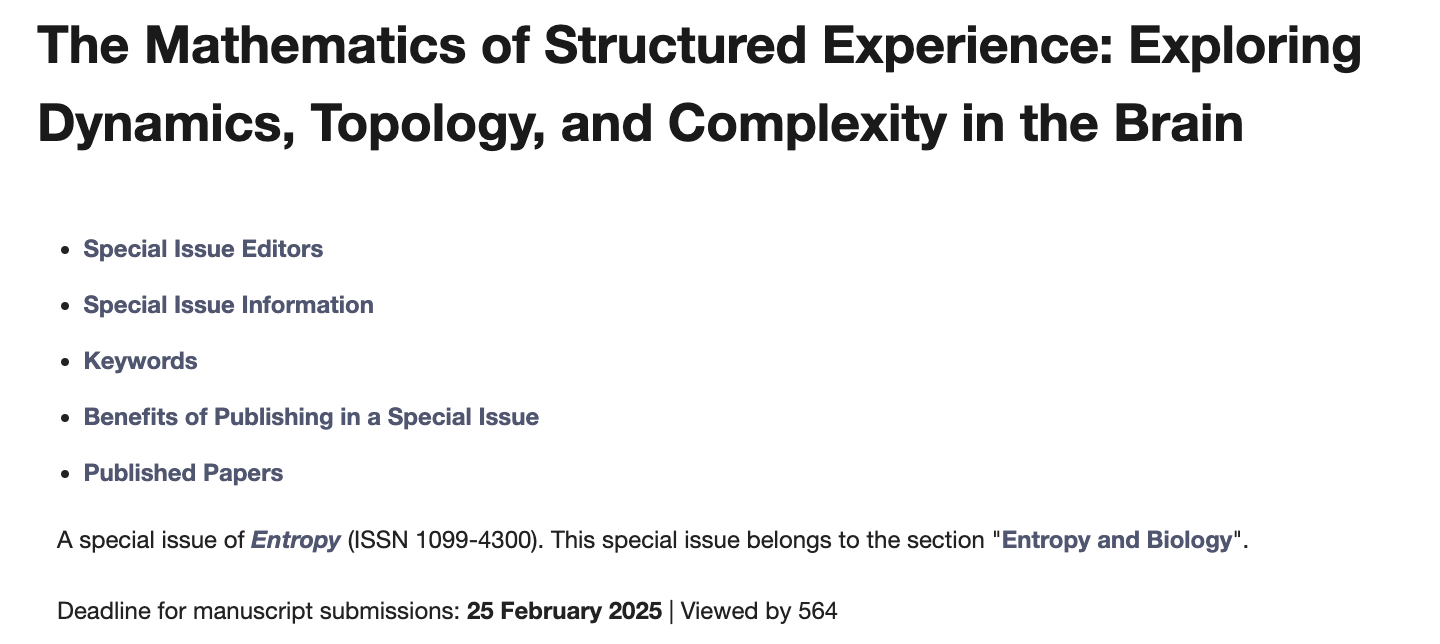
\includegraphics[width=0.75\linewidth]{image8.png}
    \end{figure}
        
   % Titled “The Mathematics of Structured Experience: Exploring Dynamics, Topology, and Complexity in the Brain”, this Special Issue aims to explore several key areas in this program:

%Characteristics of compressive world models;  We aim to delve into the nature of the world models created and run by natural and artificial agents. What do we mean, precisely, by a world model? What is the connection between program structure and the resulting dynamics? What is the role of symmetry and criticality in shaping world models and programs, and how do they enable agents to encapsulate the world's complexity in a comprehensible form?
\textbf{Topics}: Characteristics of compressive world models; Mapping models to dynamical systems;  
%A crucial exploration will be how compressive world model characteristics translate into the workings of agents as dynamical systems and their features, especially recurrent neural networks. Topics include the study of geometry and topology of invariant manifolds, dimensionality reduction (manifold hypothesis), dynamical latent spaces, and their connection with algorithmic concepts such as compression and symmetry. We invite contributions that use tools from dynamical systems theory, geometry, topology, and criticality to characterize and understand the underlying dynamics of biological or artificial systems and their relation to the data they generate (neuroimaging/neurophysiology or other data).
Empirical paradigms for validation; 
%This Special Issue also seeks to address the design of experimental paradigms aimed at validating these concepts. Specifically, we are interested in establishing connections between features derived from structured experience reports or other behavior and the observed structure in the brain (or, more generally, complex systems) dynamics (e.g., as measured by neuroimaging techniques) using the tools mentioned in the previous points. Application areas include the study of states of consciousness and disorders of consciousness, as well as non-human consciousness, using currently available datasets or through the design of specific experiments.
Implications for the design of AI and computational models of the brain. %How does this perspective influence research on artificial systems or computational models of the brain? What are the design principles inspired by the mathematics of algorithmic agenthood that can be used in artificial intelligence or computational neuroscience? 
\end{frame}
%%%%%%%%%%%%%%%%%%%%%%%%%%%%%%%%%
\begin{frame}[label=ladila]{Thanks}
\vfill
\begin{center}

   {\Large Thanks for your attention and curiosity!}  \vfill
   
  % {\large Thanks to  Ed and Roser for all the brainstorming.}  \vfill
    

    
    Slides available at {\small  %https://github.com/giulioruffini/Ruffini-KT-Tucson-presentation-April-19-2022
    https://github.com/giulioruffini/SLIDES-KT-Bamberg-presentation-Oct-2024} 
    %\\ $\rightarrow$~Preprint is on the way.
    %\vspace{1.5cm} 
    
        %giulio.ruffini@neuroelectrics.com, @ruffini (Twitter)  \vfill
        \begin{figure}
            \centering
            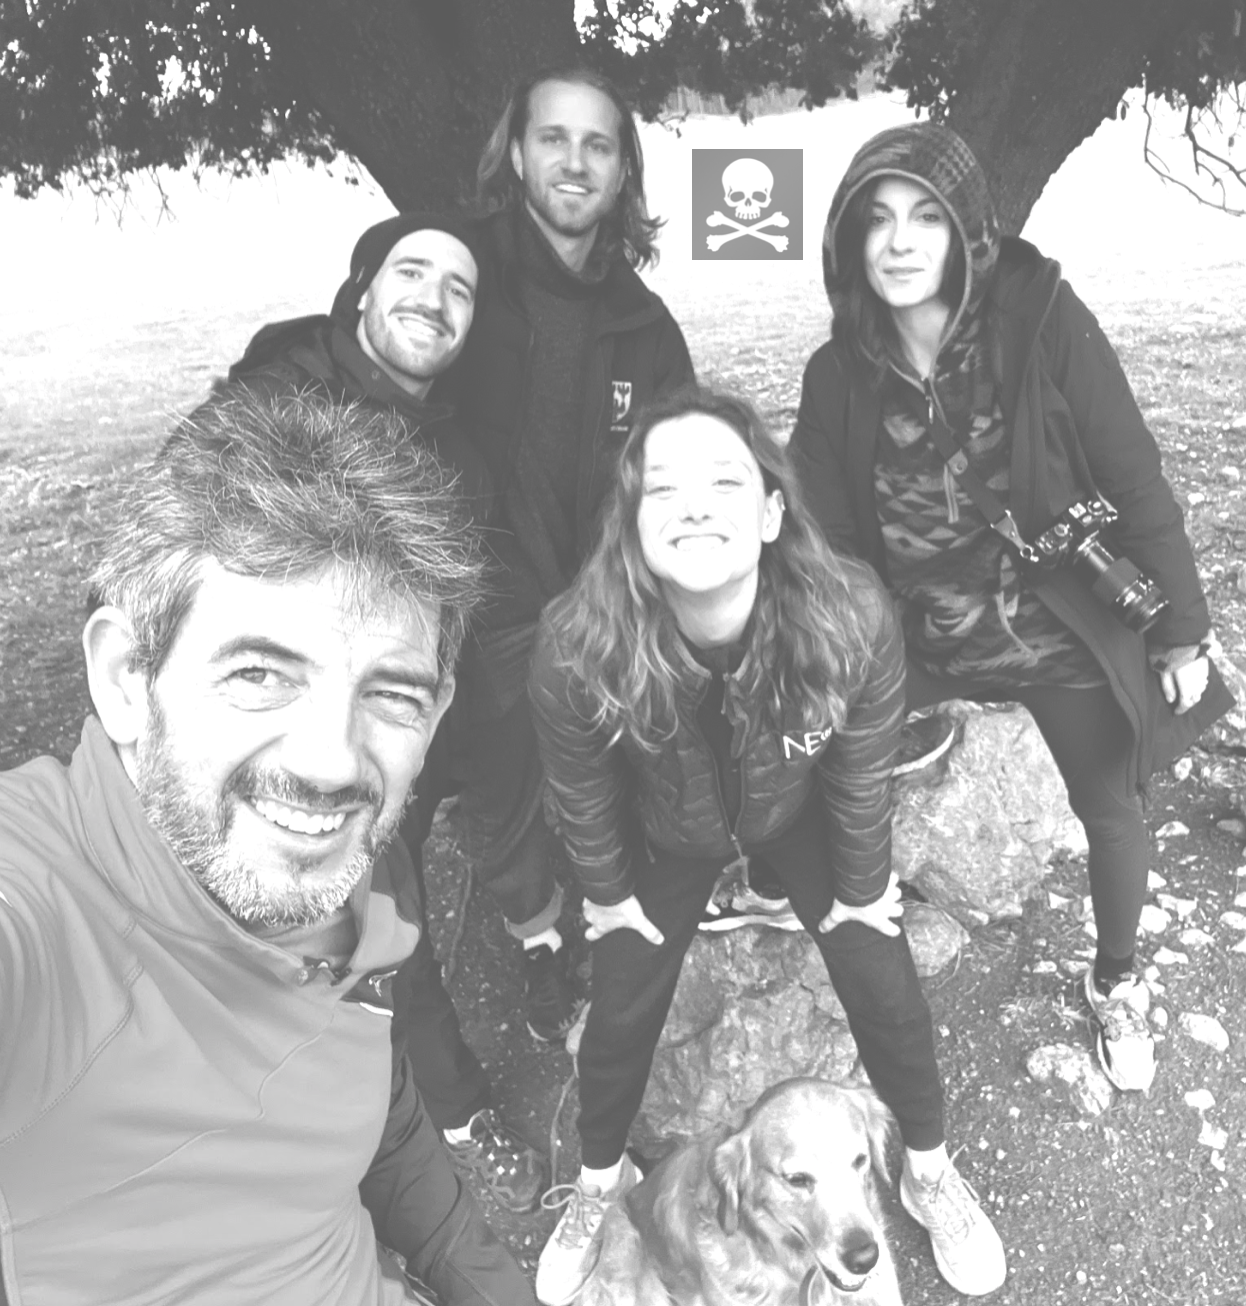
\includegraphics[width=0.33\linewidth]{image2.png}
        \end{figure}
\end{center}
\vfill

\end{frame}